\documentclass{article}
\usepackage[utf8]{inputenc}
\usepackage{amsmath}
\usepackage{graphicx}
\title{Ball Beam Balance}
\author{Qazi Umer Jamil, Mudassar Wajid}
\date{January 2016}

\usepackage{natbib}
\usepackage{graphicx}

\begin{document}

\maketitle

\section{Introduction}
We used a simple four bar mechanism, a Golf ball, and a DC motor for our setup. The design parameters in our proposal were
\[Settling time(T_s) = 3 sec\]
\[Percentage Overshoot < 8\]
\section{Mathematical Modelling of system}
Since the system actually composed of a Ball Beam balance a DC Motor, the mathematical modelling is done separately for ball beam and the motor.
\subsection{Mathematical Model of Ball Beam}
Figure 1 shows the Physical setup of our system.
\begin{figure}[h]
  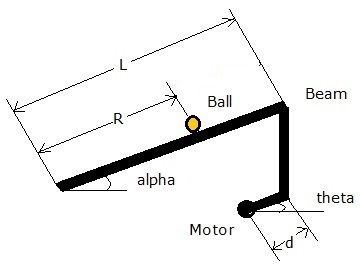
\includegraphics[width=\linewidth]{model.jpg}
  \caption{Physical Setup}
  \label{fig:boat1}
\end{figure}

The Lagrangian of any system is a quantity which can be defined as
\begin{equation} \label{eq:1}
L = K - U
\end{equation}
The kinetic energy of beam is given by
\begin{equation} \label{eq:1}
K_1 = \frac{J \alpha’^2}{2}
\end{equation}
The kinetic energy of Ball is given as
\begin{equation} \label{eq:1}
K_2 = \frac{J_b \alpha_b'^2}{2} + \frac{m v_b^2}{2}
\end{equation}
\begin{figure}[h]
  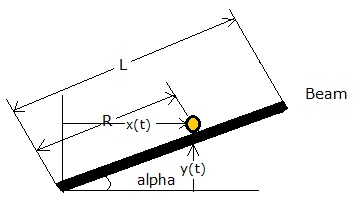
\includegraphics[width=\linewidth]{lang_fig.jpg}
  \caption{Cartesian coordinates and generalised coordinates}
  \label{fig:boat1}
\end{figure}

\[ \alpha_b'\] is the angular velocity of ball and \[v_b\] is the liner velocity of ball. In terms of generalised coordinates(as shown in figure 2), they are both related as follows:

\begin{equation} \label{eq:1}
\theta_b' = \frac{R}{r} 
\end{equation}
Where R is distance of ball from one side of the beam.
Now, we will express \[v_b\] in terms of generalised coordinates.

\begin{equation} \label{eq:1}
v_b^2 = x'^2 + y'^2;
\end{equation}

\begin{equation} \label{eq:1}
x= R\cos(\alpha)
\end{equation}

\begin{equation} \label{eq:1}
x' = R'\cos(\alpha)-R\alpha'sin(\alpha)
\end{equation}

\begin{equation} \label{eq:1}
x'^2 = R'^2 \cos^2(\alpha) - 2R'R\alpha' \cos(\alpha) \sin(\alpha) + R^2 \alpha'^2 \sin(\alpha)
\end{equation}

\begin{equation} \label{eq:1}
y= R\sin(\alpha)
\end{equation}

\begin{equation} \label{eq:1}
y' = R'\sin(\alpha)+R\alpha'cos(\alpha)
\end{equation}

\begin{equation} \label{eq:1}
y'^2 = R'^2 \sin^2(\alpha) + 2R'R\alpha' \cos(\alpha) \sin(\alpha) + R^2 \alpha'^2 \cos(\alpha)
\end{equation}

Substituting equation (8) and (11) into (5), we have
\begin{equation} \label{eq:1}
v_b'^2= R'^2 + R^2 \alpha'^2
\end{equation}

Substituting equations (12) and (4) into (3)

\begin{equation} \label{eq:1}
k_2 = \frac{1}{2} (\frac{J_b}{r^2} + m) p'^2 + \frac{1}{2}m R^2 \theta'^2
\end{equation}

The potential energy of system s given by

\begin{equation} \label{eq:1}
U = m g R \sin(\alpha)
\end{equation}

Substituting equations (2), (13), and (14) into (1), the Lagrangian for this system is

\begin{equation} \label{eq:1}
L = \frac{1}{2} (\frac{J_b}{r^2} + m) R'^2 + \frac{1}{2}(m R^2 + J) \alpha'^2 - mgR\sin(\alpha)
\end{equation}

The first Lagrange of above equation is given by

\begin{equation} \label{eq:1}
\frac{d}{dt} (\frac{\partial L}{\partial R'}) - \frac{\partial L} {\partial R} = 0
\end{equation}

Which results in

\begin{equation} \label{eq:1}
0 =  (\frac{J_b}{r^2} + m) R'' + mg\sin(\alpha) - mR\alpha'^2
\end{equation}

Linearized the above equation at \[\alpha = 0\]

\begin{equation} \label{eq:1}
  (\frac{J_b}{r^2} + m) R'' = - mg\theta 
\end{equation}
As, from Figure 1, \[\alpha = \theta \frac{d}{L} \]
So,
\begin{equation} \label{eq:1}
  (\frac{J_b}{r^2} + m) R'' = - mg\frac{d}{L} \theta
\end{equation}

Taking Laplace Transform of above equation

\begin{equation} \label{eq:1}
  (\frac{J_b}{r^2} + m) s^2 R(s) = - mg\frac{d}{L} \theta(s)
\end{equation}
Rearranging,

\begin{equation} \label{eq:1}
P(s)_b = \frac{R(s)}{\theta(s)} = \frac{-mgd}{L (\frac{J_b}{r^2} + m) s^2} 
\end{equation}

We assume that there is no slippage between ball and the beam as the ball moves, so b = 0. The system parameters of our system are as follows:
\[ m = 0.04593 kg\]
\[ R = 0.0427 m\]
\[ J = \frac{2mR^2}{5} \]
\[ g = -9.8 ms^-2 \]
\[ L = 50 x 10^2 m\]
\[ d = 3 x 10^2 m\]

Where m is the Mass of the ball, R is the Radius of ball, J is the Moment of Inertia of Ball, g is gravitational acceleration, L is Length of beam and d is lever arm offset.

After putting values in equ(21), the Transfer Function can be found as

\begin{equation} \label{eq:1}
P(s)_b = \frac{0.525}{s^2}
\end{equation}

\subsection{Mathematical Model of DC Motor}
The dynamic equation for DC motor are given as

\begin{equation} \label{eq:1}
  s(Js+b) \theta(s) = KI(s) 
\end{equation}
\begin{equation} \label{eq:1}
  (Ls+R_a) Is) = V(s) -Ks\theta(s)
\end{equation}
Rearranging above equations, we have
\begin{equation} \label{eq:1}
 P(s)_b = \frac{K}{s((Js+b)(Ls+R_a)+K^2)} 
 \end{equation}
Where \[K = K_t = K_b\]

The system parameters of motor used are as follows.
\[w_n = 3900 \frac{2 \pi}{60} rads^-1\]
\[T_s = 10.8x10^-3 Nm\]
\[I_s = 0.22 A\]
\[e_a = 24\]
\[k_b = e_a/w_n;\]
\[K_t = k_b; \]
\[R_a = K_t \frac{e_a}{T_s}\]
\[m_1 = 51x10^-3 kg\]
\[r_1 = 30.8x10^-3 m\]
\[J_1 = \frac{m_1 r_1^2}{2}\];
\[L_1 = 0\]
\[b = 0\]
All the above value were obtain from the Motor Data sheet. The DC Motor we used has model number RK-370C-081050.

Where \[w_n\] is no-load speed, \[T_s\] is stall torque, \[I_s\] is stall current, \[e_a\] is DC Operating voltage, \[R_a\] is armature resistance which is found to be \[130\Omega\], \[r_1\] is the radius of motor, \[m_1\] is the mass of motor, \[J_1\] is the moment of inertia, \[L_1\] is the armature inductance. Here our assumptions are \[b=0\] and since \[L_1<<R_a\], so \[L_a=0\]

The transfer function was found to
\begin{equation} \label{eq:1}
P(s)_m = \frac{0.05876}{  0.003159 s^2 + 0.003453 s}
 \end{equation}
 

\section{Controller Design for Ball Beam Balance}

\subsection{Using Root Locus}
Te root locus of eq(22) is shown in Figure 3. The uncompensated system has two poles at origin and no zero.
\begin{figure}[h]
  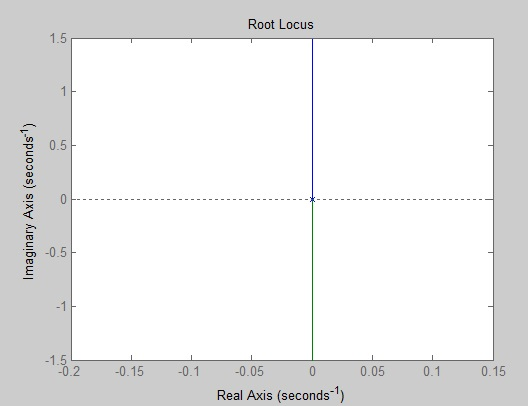
\includegraphics[width=\linewidth]{root_locus_uc.jpg}
  \caption{Root Locus of uncompensated system}
  \label{fig:boat1}
\end{figure}

To find the dominant pair of poles, we have
\[ OS = 0.08\]
This give us \[ \zeta = 0.62 \]
\[ T_s = 3 sec\]
So, 
\[ \sigma = 4/T_s = 4/3 = 1.33\]

Also, 
\[ \theta = \arctan(0.62)\]
\[ \theta = 31.79\]

And 
\[w_d = \sigma \tan(31.79)) = 1.68\]

So, the pair of our dominant poles are located at -1.33 + 1.68j

We begin designing PD Compensator. The sum of angles from the 
uncompensated system’s poles can be found as
\[\theta_1 = 180 – \theta \]
\[\theta_2 = 180 – \theta \]
Sum of angles : \[-128.32 -128.32 = -256.64\]
Thus, the contribution required from the compensator zero is 
\[180 – 268.86 = 76.64\]
From figure, we can find the location of compensator zero.
%%fig 4
\begin{figure}[h]
  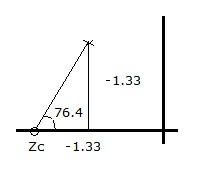
\includegraphics[width=\linewidth]{zero_pd.jpg}
  \caption{Finding zero of compensated system}
  \label{fig:boat1}
\end{figure}

\[\tan(76.64) = \frac{1.68}{z_c - 1.33}\]
\[ z_c = 1.33 + \frac{1.68}{\tan(76.64)} \]

Thus the PD Controller is (s + 1.72)

The root locus of compensated system is shown in Figure 5.

%%Fig 5
\begin{figure}[h]
  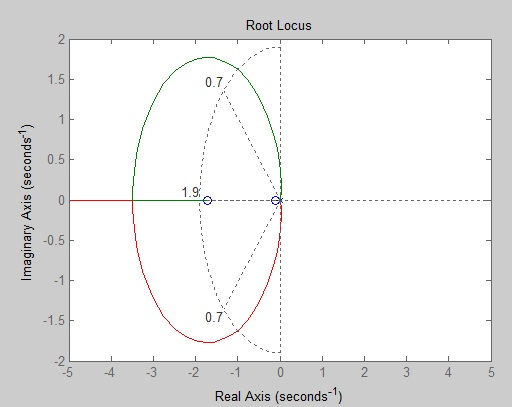
\includegraphics[width=\linewidth]{root_locus_comp.jpg}
  \caption{Root Locus of compensated system}
  \label{fig:boat1}
\end{figure}

The simulation of PD compensated system is shown in Figure 6.

%%Fig 6
\begin{figure}[h]
  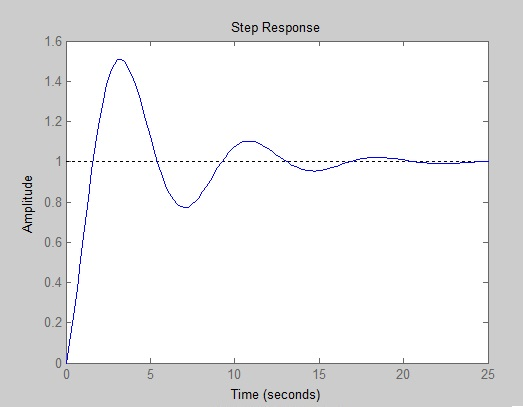
\includegraphics[width=\linewidth]{sim_com.jpg}
  \caption{Step Response of compensated system}
  \label{fig:boat1}
\end{figure}

The compensated system has Settling Time 18.7604 sec and percentage overshoot of 50.8605. The simulation shows that the require parameters cant be met. I actually have tried to design it with root locus/PID but each-time I was unable to achieve the required system response. So the other option we have using Ziegler–Nichols Method to find the value of or constants.

\subsection{Using Ziegler–Nichols Method}
Using Ziegler–Nichols method and tinkering with values of Kp, Ki, Kd, we achieve the desired response of our system. 

The settling Time is 2.58 and Overshoot: 4.57 for kp =10, ki =0, kd =15. Thus the desired response has been achieved.

The step response of our system is shown in Figure 7.
%%Fig 7
\begin{figure}[h]
  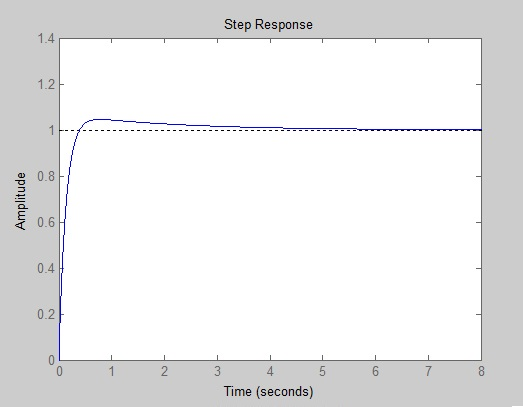
\includegraphics[width=\linewidth]{step_nz.jpg}
  \caption{Step Response of Tuned System}
  \label{fig:boat1}
\end{figure}


\section{Controller Design of DC Motor}
 
 Using Nichlus Zigler tunning method, the PID coefficients can be found as
\[Kp = 10;\]
\[Kd = 5;\]
\[Ki = 3;\]
The compensated system has Settling Time of 0.0383 and Overshoot of 0.8116, which suits our requirement.
The step response of this system is shown in Figure 8.
%%Fig 8
\begin{figure}[h]
  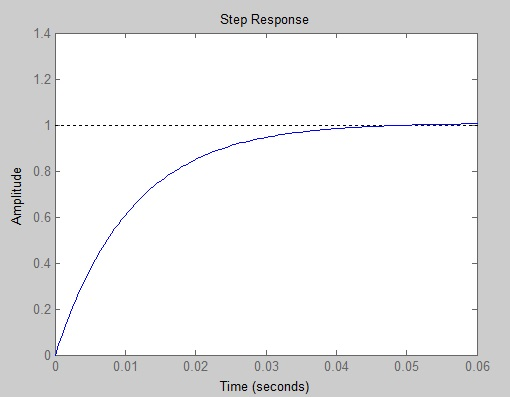
\includegraphics[width=\linewidth]{motor_resp.jpg}
  \caption{Step Response of Motor}
  \label{fig:boat1}
\end{figure}

\section{Feedback}
We used Analogue distance sensor GP2Y0A21. This sensor has a range of 10 cm to 80 cm and it has analogue output.

For Obtaining the relation between the sensor output voltage and distance being measured, we refer to the data-sheet of our sensor(GP2Y0A21). From the data sheet, the distance measuring characteristic(output) of the sensor is shown in Figure 9.

%%Fig 9
 \begin{figure}[h!]
  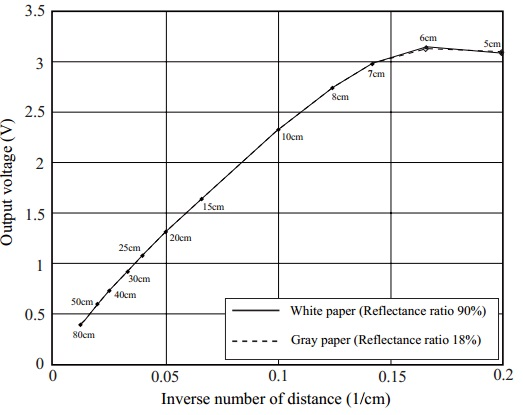
\includegraphics[width=\linewidth]{sensor.jpg}
  \caption{Output characteristic of GP2Y0A21 sensor }
  \label{fig:boat1}
\end{figure}
Figure 9 graph between the output voltage and inverse of distance shows the value of voltage for given inverse of measured distance. The average slop from point 80cm to 10cm was found to be 27. So, we can implement the sensor in Simulink in terms of following function
\[ Voltage = 27 (\frac{1}{distance})\]
This voltage will represent the voltage for a particular ball position

\section{Simulink}

The complete model of system in Simulink is shown in Figure 10.
%%Fig 9
 \begin{figure}[h!]
  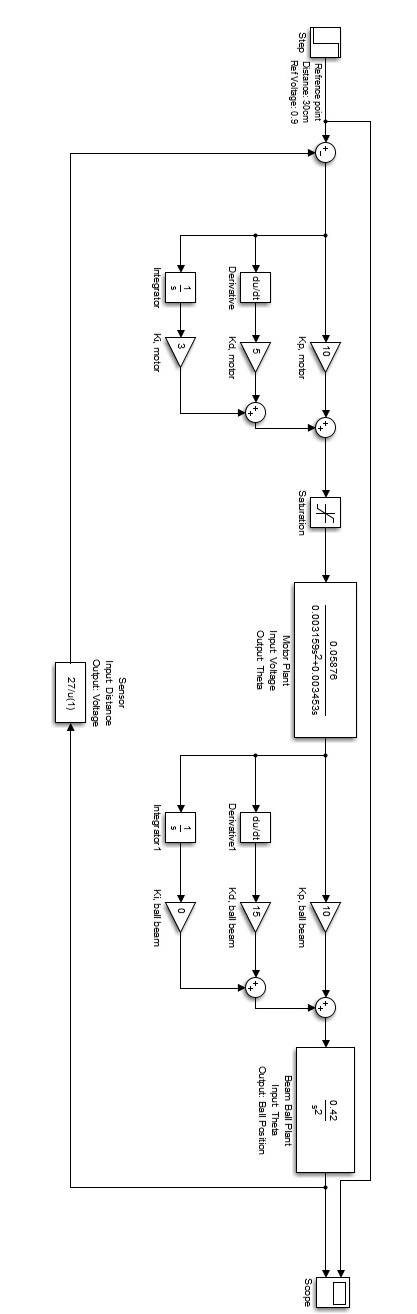
\includegraphics[scale=0.7]{simulink2.jpg}
  \caption{Simulink model of the system }
  \label{fig:boat1}
\end{figure}


\end{document}
